\documentclass[11pt]{article}
\usepackage{amsmath,amssymb,color,hyperref,graphicx,pdfsync,overpic,color,epstopdf,rotating,dashrule,float,bm}
\begin{document}
\bibliographystyle{plain}

\title{\textbf{\Large APC524 Final Project:} \\ Final Report}
\author{Anthony DeGennaro, Kevin Nowland, Scott Dawson and Im\`ene Goumiri}
\date{18 January 2013}
\maketitle

\section{Project overview and goals}

% talk about goals, algorithms we use and what we use them for
Broadly speaking, the aim of this project was to design a Smoothed Particle Hydrodynamics (SPH) solver, which would be capable of evolving a variety of types of fluid flows. This document will discuss the scope of the project, the principles and governing equations of SPH, and the specific features that were implemented, and the results from testing, profiling and running the code. Specifically, the goals of this project were to create a physically realistic, accurate, and efficient SPH solver, which is capable of simulating a variety of test cases, including:
\begin{itemize}
\item Compressible or (nearly) incompressible fluids (i.e. gases or liquids)
\item Inviscid or viscous fluids of specified viscosity
\item Flows governed by gravitational body forces
\item The interaction/mixing between two fluids of different density
\end{itemize}
All of these aims were met, with the exception of simulating compressible flows (which would simply require the creation of another physics class in the current code). 

\section{Governing Equations}
Before discussing the specifics of our implementation, we provide a brief derivation and discussion of the typical governing equations that our code will be solving. More information about such methods is can be found in \cite{Mon92} and \cite{Mon05}, for example. To begin with, we consider the Euler equations

\begin{align}
&\frac{d\rho}{d t} + \rho\nabla \cdot  \left( \bm{u}\right)=0\label{eq:NSE1}\\
&\frac{d\bm{u}}{d t}=-\frac{1}{\rho}\nabla P\label{eq:NSE2},
\end{align}
which respectively satisfy conservation of mass and momentum for a fluid, where $\rho$ is density, $P$ is pressure, and $\bm{u}$ is velocity. Here we use the total (Lagrangian) derivative $\frac{d}{dt} = \frac{\partial}{\partial t} + \bm{u} \cdot \nabla $, and for simplicity we are neglecting the influence of body forces (such as gravity) and dissipative forces (i.e. viscosity), though we note that these will be added to our code. Any computational fluids solver must approximate these  equations in order to give a form which is amenable to numerical solution. To describe SPH, we begin by considering some domain $\Sigma$, which we parametrize by $\bm{r}$, and looking at some field $A(\bm{r})$ on this domain (which typically could be a scalar field such as $\rho$, or vector field such as $\bm{u}$.  We can first make the trivial observation that
\begin{equation}
\label{eq:1}
 A(\bm{r}) = \int_{\Sigma(\bm{s})} A(\bm{s}) \delta(\bm{r}-\bm{s}) dV.
\end{equation}

The main idea behind SPH is that we can approximate the Dirac-delta function by some smooth function W, which we refer to as a kernal, satisfying the conditions
$$  \int_{\Sigma} W(\bm{r}, h) dV = 1, \ \ \ \text{and} \ \ \    \lim_{h \rightarrow 0} W(\bm{r}, h) = \delta(\bm{r}). $$
Here $h$ can be thought of as  smoothing length, which governs the resolution of the simulation. With this approximation, \ref{eq:1} becomes
\begin{equation}
\label{eq:2}
 A(\bm{r}) = \int_{\Sigma(\bm{s})} A(\bm{s}) W(\bm{r}-\bm{s},h) dV.
\end{equation}
We proceed by making the further approximation of replacing this integral by a finite sum, where we discretise the domain into volume elements of size $(\Delta V)_i$ at location $\bm{r}_i$, and sum over these elements rather than integrating. Unlike fixed grid based solvers, in SPH we let these volume elements  move with the fluid itself, so we may think of them as discrete particles or `clumps' of fluid. We now have 
\begin{equation}
\label{eq:3}
 A(\bm{r}) = \sum_{i} A(\bm{r}_i) W(\bm{r}-\bm{r}_i,h) (\Delta V)_i = \sum_{i} A(\bm{r}_i) W(\bm{r}-\bm{r}_i,h) \frac{m_i}{\rho_i},
\end{equation}
where $m_i = \rho_i (\Delta V)_i$ is the mass of fluid particle $i$. In order to approximate the spatial gradient of the field $A$ at the location of a given fluid particle $a$, we have
\begin{equation}
\label{eq:gradient}
\nabla A(\bm{r})|_{\bm{r}_a} = \frac{\partial}{\partial \bm{r}} \sum_{i} A(\bm{r}_i) W(\bm{r}-\bm{r}_i,h) \frac{m_i}{\rho_i} = \sum_{i} A(\bm{r}_i) \frac{m_i}{\rho_i} \nabla_a W_{ai},
\end{equation}
where we use the shorthand notation $W_{ai} = W(\bm{r}_a - \bm{r}_i,h)$, and $\nabla_a$ indicates that we are taking the gradient with respect tot the coordinates of $a$.

The computation of the relevant fields over time (such as $\rho$ and $\bm{u}$) then involves computing the quantities in equations \ref{eq:NSE1} and \ref{eq:NSE2} by these approximations. For conservation of mass, we have:
\begin{align}
\frac{d\rho}{d t}  &= - \rho\nabla \cdot   \bm{u}\nonumber\\
			& = -\nabla \cdot \rho \bm{u} + \bm{u} \cdot \nabla \rho, \ \ \ \text{thus for particle $a$,}\nonumber \\
\frac{d\rho_a}{d t}	& = -  \sum_{i} \frac{m_i}{\rho_i} (\rho_i \bm{u}_i) \cdot \nabla_a W_{ai} + \bm{u}_a \cdot  \sum_{i} \frac{m_i}{\rho_i} \rho_i \nabla_a W_{ai}\nonumber\\
			& = -  \sum_{i} m_i (\bm{u}_i - \bm{u}_a) \cdot  \nabla_a W_{ai}.\label{eq:SPHCONT}
\end{align}
Similarly for conservation of momentum:
\begin{align}
\frac{d\bm{u}}{d t} &=-\frac{1}{\rho}\nabla P\nonumber\\
			& = - \frac{P}{\rho^2} \nabla\rho - \nabla\left(\frac{P}{\rho} \right), \ \ \ \text{and so}\nonumber\\
\frac{d\bm{u}_a}{d t} 	& = -  \frac{P_a}{\rho_a^2} \sum_{i} \frac{m_i}{\rho_i} \rho_i  \nabla_a W_{ai} - \sum_{i} \frac{m_i}{\rho_i} \frac{P_i}{\rho_i} \nabla_a W_{ai} \nonumber\\
			& =  - \sum_{i} m_i \left( \frac{P_a}{\rho_a^2}+ \frac{P_i}{\rho_i^2} \right)\nabla_a W_{ai}.\label{eq:SPHMOM}
\end{align}
We note that changing the form of \ref{eq:NSE1} and \ref{eq:NSE2} before applying our approximations gives a resulting formulation with smaller error than if we had applied them directly. To add viscous damping to the simulation, equation \ref{eq:SPHMOM} becomes 
\begin{equation}
\frac{d\bm{u}_a}{d t} =  - \sum_{i} m_i \left( \frac{P_a}{\rho_a^2}+ \frac{P_i}{\rho_i^2} + \Pi_{ai} \right)\nabla_a W_{ai},
\end{equation}
where the viscosity $\Pi_{ai}$ takes the form \cite{Mon94}:

\begin{equation}
\Pi_{ai}  =\begin{cases}
   \frac{ -\alpha \mu_{ai}+\beta \mu_{ai}^2}{\bar{\rho_{ai}}} & \text{\ \ if $\bm{v_{ai}}\cdot\bm{r_{ai}}<0$}\\
    0, & \text{\ \ otherwise,} 
  \end{cases}
\end{equation}
where $\mu_{ai} = \frac{h \mathbf{v}_{ai} \cdot \mathbf{r}_{ai}}{\mathbf{r}_{ai}^2+\eta^2}$, and $\alpha$, $\beta$ and $\eta$ are parameters which depend on the fluid being simulated (typically $\beta =0$ for an incompressible fluid, for example). It can similarly be shown that the SPH equivalent of the energy equation (again for an inviscid fluid) is
\begin{equation}
\frac{d\bm{e}_a}{d t} = - \frac{P_a}{\rho_a} \sum_{i} \frac{m_i}{\rho_i}(\bm{u}_i - \bm{u}_a)  \cdot \nabla_a W_{ai}\label{eq:SPHEN},
\end{equation}
where $\bm{e}_a$ is the internal energy of fluid particle $a$, though when the fluid considered is incompressible, the energy is decoupled from the momentum equation (as pressure is independent of temperature), so is not required. It should be noted here that the most relevant and accurate formulation and implementation of these equation will be dependent on the type of simulation being performed. For example, in the case of simulating a liquid, which typically has negligible density variations, and equation of state of the form
\begin{equation}
P = B\left(\left(\frac{\rho}{\rho_0}\right)^{\gamma}-1\right),
\end{equation}
can typically be used, where $\rho_0$ is a reference density, $\gamma \sim 7$, and $B$ is chosen such that density fluctuations are sufficiently small \cite{Mon05}. For simulations that involve rigid boundaries, the boundary conditions can be enforced through the creation of fixed particles along the boundary, which exert a prescribed force on the fluid particles. In our implementation, a Lennard-Jones potential force is imposed between the boundary and fluid particles, which is of the form 
\begin{equation}
f(r) = D \left(\left(\frac{r_0}{r}\right)^{p_1} - \left(\frac{r_0}{r}\right)^{p_2}\right)\frac{\bm{r}}{r},
\end{equation}
where $r_0$ is a typical particle spacing (such as the smoothing length), and $p_1$ and $p_2$ are conventionally chosen to be 12 and 6 respectively \cite{Mon94}. One downside of this implementation is that the boundary is not entirely smooth. This could be corrected for through modifying the code so that each boundary particle is also assigned a normal direction vector \cite{Mon05}, but this is beyond the scope of the present code.


In our proposed code, the equations \ref{eq:SPHCONT}, \ref{eq:SPHMOM}, and \ref{eq:SPHEN} (or a subset thereof) will be stepped forward in time from prescribed initial conditions in order to simulate the motion of the fluid with time. In practice, and in very broad terms, this involves summing up the contributions from other particles in order to determine the changes in properties of a given particle for each timestep. 
\\
% \mu_{ab} = \frac{h \mathbf{v}_{ai} \cdot \mathbf{r}_{ai}}{\mathbf{r}_{ai}^2+\eta^2}

%\section{Design Process}
%
%This section documents the process that went through in designing and writing our code. We began by talking through the   , both in terms of the physics involved and the program architecture that we planned to use. We divided up the inital workload so that each person would have . In addition to this, a single file, proof of concept code was written to quickly put together the main features and variables that our code would use. Upon writing each of the individual classes, we worked together to ensure that all could interface correctly with each other. This often involved rewriting parts of the code, or adding useful features that were originally overlooked. As the code became more complete, this phase transitioned into debugging and testing of the code as a whole. As perhaps is to be expected, many . Some of these were simple to fix, and yet others 



\section{Program Structure}

The basic program structure is shared by many integrators, and involves an 
initial set up process followed by a loop which at each iteration advances the
physical properties and writes the current state to an output file.

The initialization process involves the set up of the initial configuration of the fluid
by reading in fluid particles and their properties from one file, and if
provided, the boundary particle positions from a separate file.

The timestep loop first involves determining which particles are within the
range of influence of other particles. The physical 
properties are then advanced by the procedure outlined above. The 
integrations can be performed by any desired method of integration. The methods 
provided are Euler's method, a modified Euler method, and a predictor-corrector method.
Particle positions are outputted at regular intervals (which can be specified in the driver program \texttt{sph}) to \texttt{fluid.dat}.

\subsection{User Interface: Input}

The parameters needed to specify a particle type in the SPH method include fluid properties (such as mass, density, pressure, and energy), kinematic properties (such as position and velocity), and particle discretization properties (i.e. a particle discretization kernel function). Our main goal in designing the user interface was to develop an input protocol which would be easy to use while still allowing the user to specify many fluid properties directly. The solution we developed is quite simple: the user creates an input text file in which each of the fluid particles (along with their initial conditions) is directly specified (boundary particle locations are specified in the same way via an additional file). The proper file syntax is shown below:
%
\begin{description}
	\item[``INPUT.DAT"]
		\begin{verbatim}

[Total Number of Particles]

[Number] x y u v [Mass] [Density] [Pressure] [Energy]
                     . . . . . . .
                     . . . . . . .
		\end{verbatim}
\end{description}
 
Here, the particle numbering should begin at zero, and {x, y, u, v} specify the initial position and velocity components in a 2-D plane. The user may obviously generate the initial conditions in these input files by means of whatever pre-processing routines they desire (for example, a simple MatLab script to generate specific initial/boundary conditions often is a quick and nice solution).

Once made, the driver program \texttt{sph} can be called with the syntax
\begin{center} \texttt{sph <initFile> <boundaryFile(OPTIONAL)> <tfinal> <timestep> <integratorType> <kernelType>} \end{center}
The data files \texttt{initFile} and \texttt{boundaryFile} should be in the format shown above. The options for \texttt{<intergratorType>} are \texttt{euler}, \texttt{eulermod}, and \texttt{pc}, while the options for \texttt{<kernelType>} are \texttt{spline} and \texttt{gaussian}. The specifics of these various implementations are discussed in section \ref{Classes}.
\subsection{User Interface: Output}

Output is handled in a manner which closely resembles the input protocol. Specifically, at each timestep, the SPH code writes the full state information of each fluid particle to a pre-specified output file. The output syntax is as follows:

\begin{description}
	\item[``OUTPUT.DAT"]
		\begin{verbatim}

[Timestep 1]

[Number] x y u v [Mass] [Density] [Pressure] [Energy]
                     . . . . . . .
                     . . . . . . .

[Timestep 2]

[Number] x y u v [Mass] [Density] [Pressure] [Energy]
                     . . . . . . .
                     . . . . . . .
		\end{verbatim}
\end{description}

\subsection{Classes} 
\label{Classes} 

Perhaps the must fundamental class is \texttt{Particle}, which holds the state
of a current particle and functions to get and change that state. Each particle
is given a unique tag, and the particles have an array which contains the list 
of tags for neighboring particles. The included properties are $x$ and $y$
position, the velocities, $u$ and $v$ respectively, in those directions, the
mass of the particle, associated viscosity, as well as density and pressure
at the particle's position.

A vector of particles is included in the \texttt{Fluid} class, which contains
the overall state of the fluid. The \texttt{Fluid} also has a vector for 
boundary particles. As this is smoothed particle hydrodynamics, the particles
are smoothed out with the influence described by the kernel function. This 
function, a cubic spline or Gaussian in the provided code, is passed to 
\texttt{Fluid}. Aside from the usual get and set functions, an important
function is \texttt{Fluid::findNeighbors()}, which determines for each particle
which particles are close enough to be of influence based on the given smoothing
length. 

This \texttt{findNeighbors()} function is important for scaling, as the na\"ive
comparison of each particle to every other is an $O(n^2)$ process. To overcome
this, a mesh is temporarily imposed based on the extreme $x$ and $y$ positions
of the particles with each cell having height and width of the smoothing length.
Each particle is then placed in a grid cell. Particles are then neighbors if 
they share a grid cell or lie in adjacent cells. As long as the smoothing length
is small enough, uniform, and the particles are not densely packed, this is an 
$O(n)$ process. If all particles lie in two adjacent cells, then this can be 
$O(n^2)$, but for incompressible fluids and suitably small smoothing lengths, 
this should only occur in unphysical locations.

The \texttt{Fluid::findNeighbors()} function is the first step of the time step
loop. The \texttt{Integrator} class and its step function is then invoked. The
integrator advances the fluid properties.

The \texttt{Integrator} is passed an instance of the \texttt{Physics} class,
which contains the relevant processes to advance the fluid properties each timestep.
In the case of an incompressible fluid, these are the velocity, position and density of
each fluid particle. 
The only physics type contained within the present version of the code is \texttt{IncompVisc},
which can be used for incompressible viscous flows. The user specifies the relevant physical
paraters of the fluid - namely the coefficients in the equation of state and viscosity calculation. 
These have been set in \texttt{sph.cc} to typical values for water. Also inputted is the desired 
smoothing length, which should be about twice the typical particle spacing, and the appropriate 
gravitational force.  Originally we also had a \texttt{IncompInvisc} physics implementation, but 
this has been removed as an inviscid fluid may be simulated simply by setting the viscosity 
parameter to zero in \texttt{IncompVisc}. 

Three types of integrator are provided:
\begin{itemize}
\item \texttt{euler} A standard forward stepping Euler routine
\item \texttt{eulermod} Using the Euler method, but updating particle positions using the already
updated velocity values.
\item \texttt{predictorcorrector} A predictor corrector algorithm, based on that outlined in \cite{Price04}.
\end{itemize}
When chosing the appropriate timestep, the user must keep in mind that simulations will not necessarily `break' if the timestep is too large to be accurate, so it is important to verify that the timestep chosen is sufficiently small. This can be attained either by ad-hoc convergence testing, or with reference to the Courant condition, which states that the maximum timestep to retain accuracy is  \cite{Price04}
$$ dt_c = C_{cour} \min\left(\frac{h}{v}\right),$$
where $C_{cour}$ is a constant that is often taken to be  $0.4$, and $h$ and $v$ are typical relative particle spacings and velocities, respectively. In reality, effects such as interactions with boundaries can interfere with the validity of this condition, so we reccomend that the user verifies the accuracy of their chosen timestep. As a rule of thumb, a timestep of $0.001$ when using the \texttt{euler} method is more than sufficient for all of the testcases provided (which can be increased for the \texttt{predictorcorrector} method). 



Also included is an \texttt{Output} class which is solely used to output the
state of the fluid to an appropriate file.


\section{Testing}

Gtest was used to write tests designed to ensure that functions of the code operate as expected. Tests.cc is a driver program which runs all of the tests (which is built along with the rest of the code by the Makefile. Figure {fig:tests} shows a snippet of the output from running the tests driver program.

The tests focused on the classes \texttt{Particle}, \texttt{Fluid}, and 
\texttt{Kernel}. These classes were easiest to test as the member functions 
were simple relative to those in \texttt{Physics} and \texttt{Integrator}. The 
integrators and and types of physics had more complicated member functions
which were most easily tested through simulation once the other classes were
deemed operational. 

Once the class structure and interfaces were determined, the tests were written
and did catch several bugs. The tests proved to be more useful when changing
implementations of features to make sure the code would still run properly. This
was particularly important when rewriting \texttt{Fluid::findNeighbors()}.

\begin{figure}
\begin{center}
\includegraphics[width= 0.8\textwidth]{testexample.pdf}

\caption{Screenshot of the output of running the gtest tests.}
\label{fig:tests}
\end{center}
\end{figure}

\section{Profiling and Optimization}

Profiling was done using \texttt{gprof}. Table \ref{table:gprof} shows the
routines which took up more than 1\% of runtime when running the program
with 650 input particles and a box boundary. The routines which dominate
the program's runtime are the calculations for the physics and various gets
and sets. We were encouraged by this profile, as we found the gets and sets
to largely be necessary in object-oriented code. This does suggest that
a different repackaging of the properties to avoid these could significantly
reduce runtime.

The other main use of profiling was to determine the scaling properties of
\texttt{Fluid::findNeighbors()}. Initially, each particle's position was 
compared to the position of every other particle to determine possible
influence. This is an $O(n^2)$ algorithm. In profiling, it was found that
this function for a large number of particles took up the plurality (greater
than 30\%) of runtime. After switching to the mesh method described above,
find neighbors scaled linearly, as expected.

Initially, we planned to reduce runtime by parallelizing many of the 
calculations. In fact, the inducement of the mesh in the 
\texttt{findNeighbors} method suggests that one way to do this would be
to partition the domain based on the temporary grid. This would allow not
only for the easy OpenMP parallelization of for loops, but to use the more 
versatile MPI.

\begin{table}
  \centering
  \texttt{
  \begin{tabular}{|c|c|c|c|}
    \hline 
    \% time & cum. seconds & self seconds & name \\
    \hline
    36.61&33.61&33.61&IncompVisc::rhs\\
    \hline
    25.23&56.77&23.16&Fluid::getParticles\\
    \hline
    18.88&74.10&17.33&Fluid::findNeighbors\\
    \hline
    9.26&82.60&8.50&Fluid::getBoundaries\\
    \hline
    5.36&87.52&4.92&Particle::getOldProperties\\
    \hline
    2.06&89.41&1.89&SplineKernel::gradW\\
    \hline
    1.38&90.68&1.27&Particle::deleteNeighbors\\
    \hline
  \end{tabular}
  }
  \caption{Table containing sample \texttt{gprof -b sph} output.}
  \label{table:gprof}
\end{table}


\section{Results}

Here some typical results from running the code in a variety of scenarios are presented. We focus on applications particularly suited to particle-based codes, such as flows with highly deforming free surfaces and mixing of fluids with different densities. We begin with a comparison with an example from the literature - a dam breaking and flowing over a triangular obstacle \cite{Mon94}. Figure \ref{fig:Comparison} shows the comparison between the results from both the previous investigation and our own code. 

Figures \ref{fig:Incline} and \ref{fig:Mixing} respectively show the results of simulating a sphere of fluid falling onto an inclined plane, and two fluids of different densities mixing in a box.

\begin{figure}
\begin{center}
(a)\includegraphics[width= 0.35\textwidth]{DamburstexampleMon94.pdf}
(b) \includegraphics[width= 0.45\textwidth]{DamburstOurcode2.eps}

\caption{Comparison between SPH results for a breaking dam flowing over a triangular obstacle from (a) the results of \cite{Mon94}, and (b) our code. }
\label{fig:Comparison}
\end{center}
\end{figure}

\begin{figure}
\begin{center}
\includegraphics[width= 0.45\textwidth]{sphereincline1.eps}
\includegraphics[width= 0.45\textwidth]{sphereincline2.eps}
\includegraphics[width= 0.45\textwidth]{sphereincline3.eps}
\includegraphics[width= 0.45\textwidth]{sphereincline4.eps}
\caption{Simulation of a sphere impinging on a 45 degree inclined plane }
\label{fig:Incline}
\end{center}
\end{figure}

\begin{figure}
\begin{center}
\includegraphics[width= 0.45\textwidth]{SpheresDiffdensities_1.pdf}
\includegraphics[width= 0.45\textwidth]{SpheresDiffdensities_201.pdf}
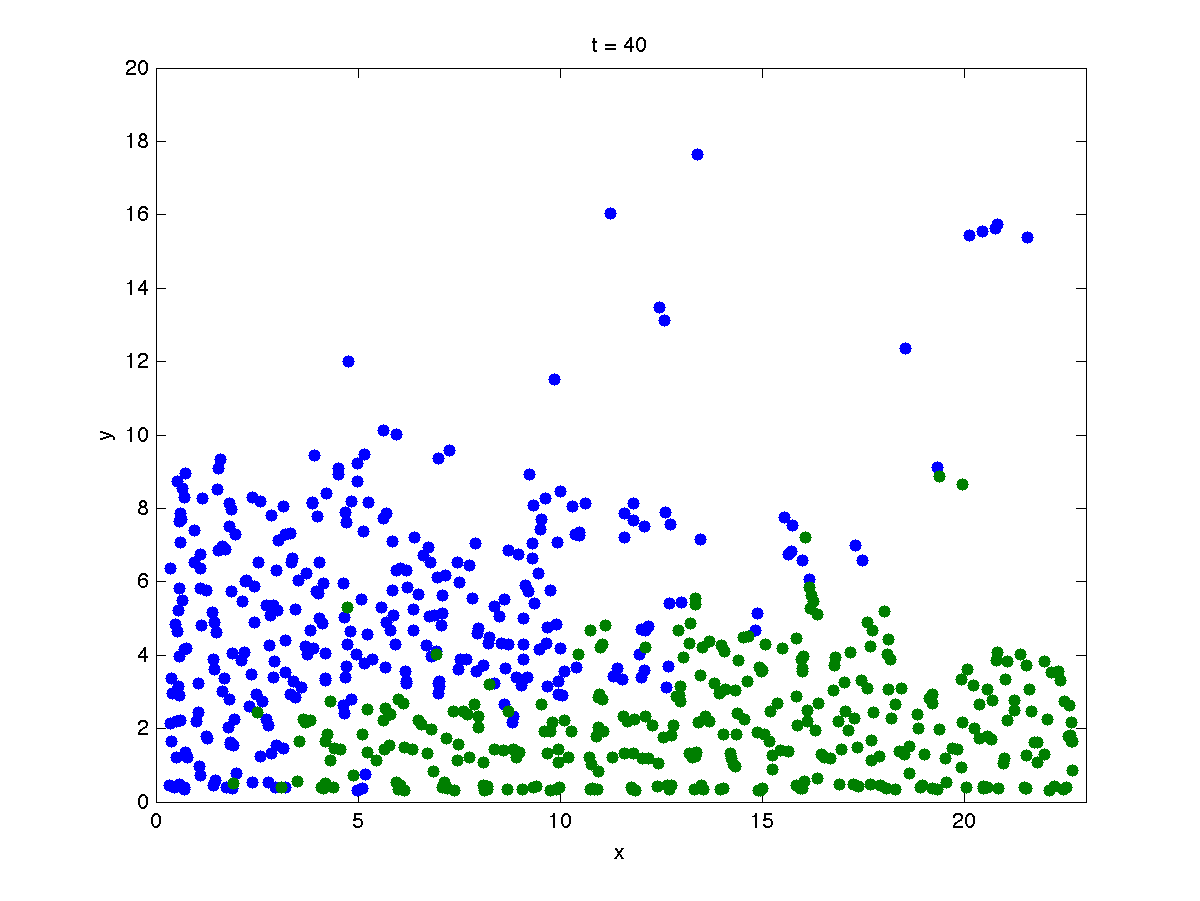
\includegraphics[width= 0.45\textwidth]{SpheresDiffdensities_401.pdf}
\includegraphics[width= 0.45\textwidth]{SpheresDiffdensities_801.pdf}
\caption{Simulation of two fluids of different densities mixing. The blue fluid is half the density of the green.}
\label{fig:Mixing}
\end{center}
\end{figure}


\section{Design Process and Lessons learned}

This section documents the process that went through in designing and writing our code. We began by talking through the main ideas of the project, in terms of the scope, the physics involved and the program architecture that we planned to use. We divided up the initial workload so that each person would have a class to begin coding. In addition to this, a single file, proof of concept code was written to quickly put together the main features and variables that our code would use. Upon writing each of the individual classes, we worked together to ensure that all could interface correctly with each other. This often involved rewriting parts of the code, or adding useful features that were originally overlooked. As the code became more complete, this phase transitioned into debugging and testing of the code as a whole. As perhaps is to be expected, many errors and limitations within our code emerged. Some of these were simple to fix, while others were significantly more elusive. 

The act of writing tests was useful not only to uncover previously undetected errors and bugs, but also to solidify our understanding of the intended functionality of each aspect of the code

Pointers tend to proliferate in object-oriented code, and memory management,
keeping track of what existed where and detecting memory leaks, became quite
difficult after a time. This led to a wholesale switch to using the
\texttt{boost} library's \texttt{shared\_ptr}. This allowed us to remove all
calls to \texttt{delete} and prevented memory leaks. The main downside for 
this is that \texttt{boost} is large and may not be installed everywhere, 
somewhat hurting the portability of the code. When \texttt{C++11} becomes
fully standard and supported, similar functionality will be available without
having to install a separate library.

\section{Further Work}
Possible extensions of the present code could include:
\begin{itemize}
\item Creation of alternative physics classes (such as to allow for compressible flows)
\item Paralization of the code, which could involve either using OpenMP to parallalize the for loop of the timestepper, for example, or using MPI with an extension of the domain decomposition technique that was used
for the findneighbors algorithm
\item Modify the code so that some functions (e.g. updating neigbors) are not performed every timestep
\item Extension to three dimensional flows (which would require significantly more work, and would probably
want to happen after the previous step)
\end{itemize}


\bibliography{refs}


\end{document}
